% Chapter Template

\chapter{Introduction} % Main chapter title

\label{Chapter1} % Change X to a consecutive number; for referencing this chapter elsewhere, use \ref{ChapterX}

\fancyhead[RO]{\thepage}
\fancyhead[RE]{\thepage}
\fancyhead[LE]{Chapter 1.~\emph{\Chaptername}}
\fancyhead[LO]{\emph{Modeling of EM Wave Propagation in NIM using FDTD}}

%----------------------------------------------------------------------------------------
%	SECTION 1
%----------------------------------------------------------------------------------------

\section{Background }
\index{NIM}
In 2000 Smith, Schultz and coworkers \cite{smith} demonstrated that it is possible to create a material artificially to have different EM  characteristics, it was the first NIM ever created. Negative Index Material (NIM) or Left Handed Material (LHM) is a material which has negative permeability and permittivity. Due to this it behaves differently as compared to naturally occurring materials. Although NIM have been introduced in 1968 \cite{vesel}
it's surprising phenomena are still not well understood in details.

 In addition
to a negative index (NI) of refraction, properties such as artificial
magnetism \cite{pendry}
, negative permittivity, and negative permeability have
been observed in fabricated NIM composites; 
Having these special characteristics NIM became ideal candidate 
for applications like Super Lens, Optical fiber cable, RADAR systems, EM absorbers.and invisibility cloaking. With
encouraging results having been demonstrated at microwave
frequencies, there has been a determined push to extend NIMs to
the terahertz, infrared, and visible bands which resulted in establishment of many
research programs, conferences, workshops, and significant
funding efforts dedicated to understanding and developing NIMs.
Since 2000, the rate of publications on EM-NIMs has grown
exponentially, \cite{rama}
indicating the increase in interest that NI
materials have generated. Much of that interest has been sparked by
the property of negative refractive index.

\begin{figure}[htbp]
	\centering
		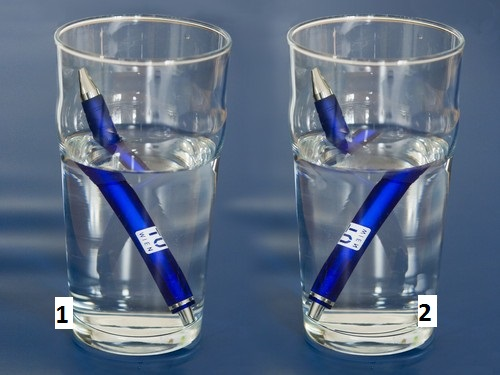
\includegraphics[width=4in]{Pictures/glass.jpg}
		\rule{35em}{0.5pt}
	\caption[Illustration of NIM]{(1) shows the normal phenomenon of refraction in water having positive value of refractive index. (2) shows the unusual phenomenon of refraction in water having negative value of refractive index}
	\label{fig:glass}
\end{figure}


%----------------------------------------------------------------------------------------
%	SECTION 2
%----------------------------------------------------------------------------------------
\index{Problem statement}
\section{Problem Statement}

To model an NIM (slab) using (frequency dependent dispersive) drude model that will effectively have refractive index of -1 (choosing $\mu_{r} = -1$ and $\epsilon_{r} = -1$ ) at 3 GHz.

Objectives of this project are 
\begin{itemize}
\item[-] To simulate and observe the behavior of Electromagnetic Waves when they pass through negative index materials
\item[-] To use FDTD algorithm and modify it for negative index material simulations
\item[-] Reducing computational time by using the parallel processing power of Graphics Processing Units (GPU)
\item[-] Comparison of algorithm performance on different platforms (MATLAB, C++, GPU)
\end{itemize}

%-----------------------------------
%	SUBSECTION 1
%-----------------------------------
%\subsection{Negative Index Material}

